\chapter{Переходные процессы}
    Уравнение Нернста-Планка
    \begin{equation}
        j = -\frac{z}{|z|}ukT\pder{n}{x} - |z|nue\pder{\phi}{x}.
        \label{eq:nernst-plank-2}
    \end{equation}
    не содержит явно времени и описывает установившийся ток, плотность которого
    одинакова по всей толщине мембраны. Получим с его помощью уравнение для
    переходного процесса. Для этого воспользуемся уравнением непрерывности:
    \begin{equation}
        \pder{\rho}{t} + \divergence\vec{j} = 0.
    \end{equation}
    Учитывая, что \( \rho = nez \), для одномерного случая получим уравнение
    \begin{equation}
        \pder{n}{t} = \frac{ukT}{e|z|}\ppder{n}{x} +
            \frac{z}{|z|}u\pder{\phi}{x}\pder{n}{x} +
            \frac{z}{|z|}u\ppder{\phi}{x}n.
        \label{eq:nernst-plank-2_with_time}
    \end{equation}
    Попробуем теперь узнать характерное время, необходимое на установление
    равновесных распределений концентраций. Для этого будем считать, что
    потенциал в начальный момент времени уже имеет равновесное
    распределение. Рассмотрим 2 простых случая, особенно часто употребляемых в
    биофизике:
    \begin{enumerate}
        \item \textbf{линейное распределение потенциала}\\
            в этом случае
            \[
                \pder{\phi}{x} = -E = \const
            \]
            и уравнение (\ref{eq:nernst-plank-2_with_time}) упрощается
            \begin{equation}
                \pder{n}{t} = \frac{ukT}{e|z|}\ppder{n}{x} -
                    \frac{z}{|z|}uE\pder{n}{x}.
            \end{equation}
        \item \textbf{линейное распределение концентрации}\\
            в этом случае сначала необходимо из уравнения
            (\ref{eq:nernst-plank-2}) получить равновесное распределение
            потенциала:
            \[
                n = n_{out} - \frac{n_{out} - n_{in}}{d} x,\ j = -\pder{z}{|z|}ukTn_1 -
                    |z|ue(n_{out}+n_1x)\pder{\phi}{x},
            \]
            \[
                \pder{\phi}{x} = -\frac{\phi_0}{\ln\frac{n_{out}}{n_{in}}}
                \frac{n_{in} - n_{out}}{d}
                \frac{1}{n_{out} - \frac{n_{out} - n_{in}}{d} x}.
            \]
            Подставляя в уравнение (\ref{eq:nernst-plank-2_with_time}), получаем
            \begin{gather}
                \pder{n}{t} = \frac{ukT}{e|z|}\ppder{n}{x} -
                \frac{z}{|z|}u\frac{\phi_0}{\ln\frac{n_{out}}{n_{in}}}
                \frac{n_{in} - n_{out}}{d}
                \frac{1}{n_{out} - \frac{n_{out} - n_{in}}{d} x}
                \pder{n}{x} + \nonumber \\
                + \frac{|z|}{z}u\frac{\phi_0}{\ln\frac{n_{out}}{n_{in}}}
                \frac{(n_{in} - n_{out})^2}{d^2}
                \frac{1}{(n_{out} - \frac{n_{out} - n_{in}}{d} x)^2}n.
            \end{gather}
    \end{enumerate}

\section{Приближение постоянного поля}
\subsection{Условие применимости}
    В приближении постоянного поля стационарное распределение концентраций,
    получаемая из уравнения Нернста-Планка, определяется зависимостью
    \[
        n(x) = \frac{(n_{out}e^\alpha - n_{in}) - (n_{out} -
        n_{in})e^{\alpha\frac{x}{d}}}{e^\alpha - 1},\ \alpha = \frac{zeEd}{kT}.
    \]
    Ионы в мембране создают поле \( E_i \), причем это поле действует и на
    сами ионы. Условием применимости может служить требование
    \[
        E_i^{max} \ll E.
    \]
    Определим поле \( E_i \). Для этого воспользуемся уравнением Максвелла
    \[
        \divergence\vec{E}_i = \pder{E_i}{x} = \frac{\rho}{\eps\eps_0}.
    \]
    Интегрируя его, получим
    \begin{gather}
        E_i(x) = E_i(0) + \frac{ez}{\eps\eps_0}\int_0^x n(\xi)d\xi = \nonumber\\
        = E_i(0) + \frac{ez}{\eps\eps_0}\left[
        \frac{n_{out}e^\alpha - n_{in}}{e^\alpha - 1}x - \frac{n_{out} -
        n_{in}}{e^\alpha - 1}\frac{d}{\alpha}{e^{\alpha\frac{x}{d}} - 1}
        \right].
    \end{gather}
    Так как поле создаётся плоскими слоями, в границах которых плотность заряда
    постоянна, то на краях мембраны поле внутренних ионов будет иметь разное
    направление, но одинаковую величину:
    \begin{equation}
        E_i(d) = -E_i(0) = E_i(0) + \frac{ez}{\eps\eps_0}\left[
        \frac{n_{out}e^\alpha - n_{in}}{e^\alpha - 1}d - \frac{n_{out} -
        n_{in}}{e^\alpha - 1}\frac{d}{\alpha}{e^\alpha - 1}
        \right].
    \end{equation}
    Отсюда находим \( E_i(0) \) и подставляем в выражение для поля:
    \begin{equation}
        E_i = \frac{ez}{\eps\eps_0}\left[
        \frac{n_{out}e^\alpha - n_{in}}{e^\alpha - 1}\left(x-\frac{d}{2}\right)
        - \frac{n_{out} - n_{in}}{e^\alpha - 1}\frac{d}{\alpha}
        \left(e^{\alpha\frac{x}{d}} - \frac{e^\alpha + 1}{2}\right)
        \right].
    \end{equation}
    Очевидно, что максимальное значение величина поля принимает вблизи краёв
    мембраны:
    \begin{equation}
        E_i^{max} = \frac{ezd}{2\eps\eps_0\alpha(e^\alpha - 1)}\left\{
            n_{out}[(\alpha - 1)e^\alpha + 1] - n_{in}[\alpha + 1 - e^\alpha]
        \right\} \ll E.
    \end{equation}
\subsection{Решение уравнения}
    Для удобства в уравнении
    \[
        \pder{n}{t} = \frac{ukT}{e|z|}\ppder{n}{x} -
            \frac{z}{|z|}uE\pder{n}{x}.
    \]
    введём следующие обозначения
    \[
        \frac{ukT}{e|z|} = D,\quad \frac{z}{|z|}uE = v.
    \]
    С учётом этого, уравнение принимает вид
    \[
        \pder{n}{t} = D\ppder{n}{x} - v\pder{n}{x}.
    \]
    Это уравнение конвективной диффузии. Поставим краевую задачу для
    этого дифференциального уравнения в частных производных -- будем
    считать концентрации на краях мембраны постоянными, так как они
    определяются концентрациями в омывающих растворах, а начальное
    условие -- нулевым, то есть будем считать, что сначала мембрана
    свободна от ионов. Задача приобретает вид
    \begin{align*}
        & \pder{n}{t} = D\ppder{n}{x} - v\pder{n}{x},\ x\in(0,d)\\
        & n(0, t) = n_{out},\ t>0 \\
        & n(d, t) = n_{in},\ t>0 \\
        & n(x, 0) = 0,\ x\in(0,d).
    \end{align*}
    Для удобства решения обезразмерим её:
    \( x = \xi d, t = \tau d^2 / D \)
    \begin{align*}
        & \pder{n}{\tau} = \ppder{n}{\xi} -
            w\pder{n}{\xi},\ w = \frac{vd}{D},\ \xi\in(0,1) \\
        & n(0, \tau) = n_{out},\ \tau>0 \\
        & n(1, \tau) = n_{in},\ \tau>0 \\
        & n(\xi, 0) = 0,\ \xi\in(0,1).
    \end{align*}
    Эта систему можно решить численно. Для этого построим явную разностную
    схему:
    \[
        \frac{n(\xi_i,\tau_{j+1}) - n(\xi_i, \tau_j)}{\Delta\tau} =
        \frac{n(\xi_{i+1},\tau_j) - 2n(\xi_i, \tau_j) +
        n(\xi_{i-1},\tau_j)}{\Delta\xi^2} -
        w\frac{n(\xi_{i+1},\tau_j) - n(\xi_{i-1}, \tau_j)}{2\Delta\xi},
    \]
    \begin{gather*}
        n(\xi_i,\tau_{j+1}) =
        [1-2r]n(\xi_i, \tau_j) +
        r\left(
            [1 - s]n(\xi_{i+1},\tau_j) + [1 + s]n(\xi_{i-1},\tau_j)
        \right),\\
        r = \frac{\Delta\tau}{\Delta\xi^2}, s = \frac{w\Delta\xi}{2}.
    \end{gather*}
    Результаты численного расчёта для иона натрия в мембране аксона кальмара
    представлены на рисунке~\ref{fig:1}.
    \begin{figure}[H]
    \begin{center}
        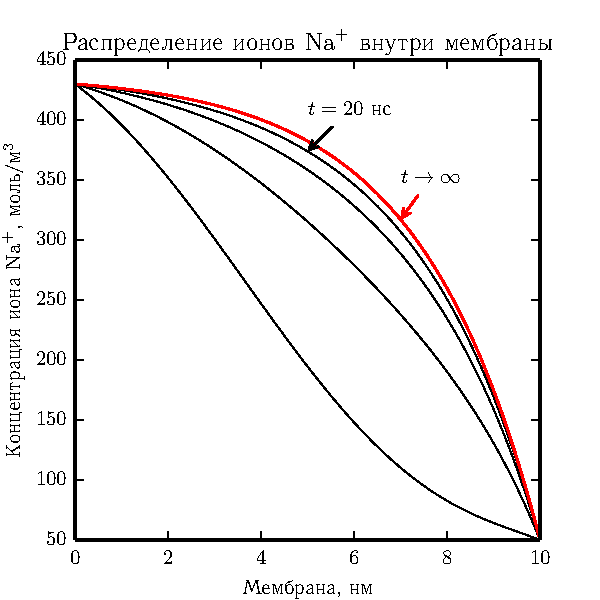
\includegraphics[width=.7\textwidth]{plots/linear_field}
    \end{center}
    \caption{Процесс установления профиля концентрации в постоянном поле. Чёрные
    кривые -- профили в различные моменты времени с шагом 5 нс, красная --
    установившийся профиль.}
    \label{fig:1}
    \end{figure}


\section{Приближение постоянного градиента концентрации}
\subsection{Условие применимости}
    Как и в приближении постоянного поля достаточно потребовать малости поля
    ионов в мембране по сравнению с внешним полем
    \[
        E = \frac{\phi_0}{\ln\frac{n_{out}}{n_{in}}}
            \frac{n_{in} - n_{out}}{d}
            \frac{1}{n_{out} - \frac{n_{out} - n_{in}}{d} x}.
    \]
    Внешнее поле принимает минимальное значение на том краю, где концентрация
    ионов больше:
    \[
        E_{min} = \frac{\phi_0}{\ln\frac{n_{out}}{n_{in}}}
            \frac{n_{in} - n_{out}}{d}\frac{1}{\max(n_{out}, n_{in})}.
    \]
    Для собственного поля ионов имеем
    \begin{gather}
        E_i(x) = E_i(0) + \frac{ez}{\eps\eps_0}\int_0^x n(\xi)d\xi = \nonumber\\
        = E_i(0) + \frac{ez}{\eps\eps_0}\left(
        n_{out} x - \frac{n_{out} - n_{in}}{d}\frac{x^2}{2}\right).
    \end{gather}
    Максимальное значение оно принимает на краях мембраны. Поле ионов имеет вид
    \begin{equation}
        E_i(x) = \frac{ez}{\eps\eps_0}\left[
        n_{out} \left(x-\frac{d}{2}\right) - \frac{n_{out} - n_{in}}{2d}
        \left(x^2 - \frac{d^2}{2}\right)
        \right].
    \end{equation}
    \begin{equation}
        E_i^{max} = \frac{ezd}{\eps\eps_0}\frac{n_{in}+n_{out}}{4} \ll E_{min}.
    \end{equation}

\subsection{Решение уравнения}
    Уравнение
    \begin{gather}
        \pder{n}{t} = \frac{ukT}{e|z|}\ppder{n}{x} -
        \frac{z}{|z|}u\frac{\phi_0}{\ln\frac{n_{out}}{n_{in}}}
        \frac{n_{in} - n_{out}}{d}
        \frac{1}{n_{out} - \frac{n_{out} - n_{in}}{d} x}
        \pder{n}{x} + \nonumber \\
        + \frac{|z|}{z}u\frac{\phi_0}{\ln\frac{n_{out}}{n_{in}}}
        \frac{(n_{in} - n_{out})^2}{d^2}
        \frac{1}{(n_{out} - \frac{n_{out} - n_{in}}{d} x)^2}n.
    \end{gather}
    можно переписать в виде
    \begin{equation}
        \pder{n}{t} = D\ppder{n}{x} - vf(x)\pder{n}{x} + \frac{v}{d}f^2(x)n,
    \end{equation}
    где
    \begin{equation}
        D = \frac{ukT}{e|z|},\ v = \frac{z}{|z|}\frac{u}{d}
        \frac{\phi_0}{\ln\frac{n_{out}}{n_{in}}},
        \ f(x) = \frac{d}{x - n_{out}d / (n_{out}-n_{in})}.
    \end{equation}
    Это уравнение с переменными коэффициентами, в котором в свою очередь можно
    уйти от конкретных размеров мембраны:
    \begin{equation}
        \pder{n}{\tau} = \ppder{n}{\xi} - wg(\xi)\pder{n}{\xi} + wg^2(\xi)n,
    \end{equation}
    где
    \begin{equation}
        \tau = \frac{D}{d^2}t,\ \xi = \frac{x}{d},\ w = \frac{vd}{D},
        \ g(\xi) = \frac{1}{\xi - \frac{n_{out}}{n_{out} - n_{in}}}.
    \end{equation}
    Опять поставим для этого уравнения краевую задачу:
    \begin{align*}
        & \pder{n}{\tau} = \ppder{n}{\xi} - wg(\xi)\pder{n}{\xi} + wg^2(\xi)n,
            \ \xi\in(0,1) \\
        & n(0, \tau) = n_{out},\ \tau>0 \\
        & n(1, \tau) = n_{in},\ \tau>0 \\
        & n(\xi, 0) = 0,\ \xi\in(0,1).
    \end{align*}
    Явная разностная схема в этом случае имеет вид:
    \begin{gather*}
        n(\xi_i,\tau_{j+1}) =
        [1-2r+qg^2(\xi)]n(\xi_i, \tau_j) +\\
        + r\left(
            [1 - sg(\xi_i)]n(\xi_{i+1},\tau_j) +
            [1 + sg(\xi_i)]n(\xi_{i-1},\tau_j)
        \right),\\
        r = \frac{\Delta\tau}{\Delta\xi^2}, s = \frac{w\Delta\xi}{2},
        q = w\Delta\tau.
    \end{gather*}
    Результат численного решения для иона натрия в мембране аксона кальмара
    представлен на рисунке~\ref{fig:2}.
    \begin{figure}[H]
    \begin{center}
        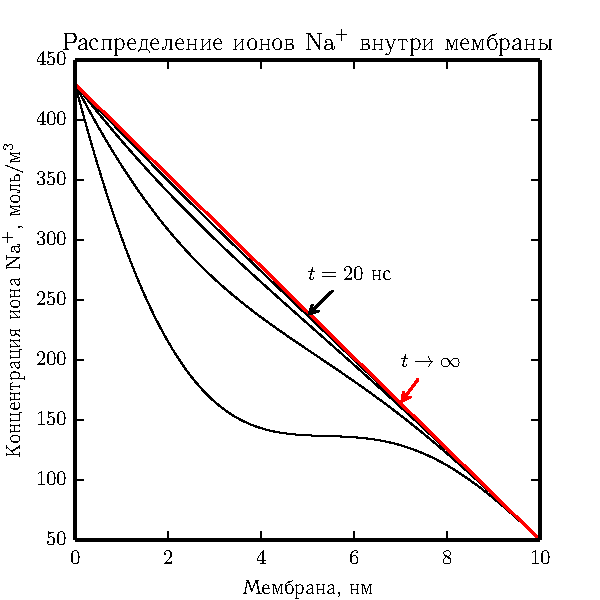
\includegraphics[width=.6\textwidth]{plots/linear_conc}
    \end{center}
    \caption{Процесс установления линейного профиля концентрации. Чёрные кривые
    -- профили в различные моменты времени с шагом 5 нс, красная --
    установившийся линейный профиль.}
    \label{fig:2}
    \end{figure}

    Таким образом, за время порядка \(10^{-8}\) -- \(10^{-7}\) с в обоих
    рассмотренных приближениях устанавливается равновесное распределение
    концентраций.

\section{Учёт поля ионов}
    Запишем снова уравнение Нернста-Планка:
    \begin{equation}
        j = -\frac{z}{|z|}ukT\pder{n}{x} + |z|nueE.
    \end{equation}
    Поле \( E \) складывается из нескольких компонент: внешнего поля и полей,
    создаваемых каждым из сортов ионов в мембране.
    \begin{equation}
        E = E_{ex} + \sum_{i} E_i.
    \end{equation}
    Рассмотрим случай пассивного транспорта ионов одного сорта. В этом случае
    \begin{equation}
        E = E_{ex} + E_{in}.
    \end{equation}
    Так как задача плоская, то внешнее поле может быть только однородным.
    Электрическое поле ионов связано с их концентрацией уравнением Максвелла:
    \begin{equation}
        \pder{E_{in}}{x} = \frac{nez}{\eps\eps_0},\quad
        n = \frac{\eps\eps_0}{ez}\pder{E_{in}}{x}.
    \end{equation}
    Тогда плотность ионного тока определяется выражением
    \begin{equation}
        j = \eps\eps_0
            \left(-D_i\ppder{E_{in}}{x}+\frac{z_i}{|z_i|}u_iE\pder{E_{in}}{x}\right).
        \label{eq:j_from_E}
    \end{equation}
    Теперь воспользуемся уравнением непрерывности:
    \begin{equation}
        \pder{\rho}{t} + \pder{j}{x} = 0.
    \end{equation}
    Выразим плотность заряда из уравнения Максвелла и подставим в уравнение
    непрерывности:
    \begin{equation}
        \pder{E_{in}}{x} = \frac{\rho}{\eps\eps_0},\quad
        \eps\eps_0\pder{}{t}\pder{E_{in}}{x} + \pder{j}{x} = 0.
    \end{equation}
    Отсюда
    \begin{equation}
        \pder{}{x}\left(\eps\eps_0\pder{E_{in}}{t} + j\right) = 0,
    \end{equation}
    \begin{equation}
        \pder{j}{x} = -\eps\eps_0\pcder{E_{in}}{x}{t}.
        \label{eq:displacement-current}
    \end{equation}
    Подставляя \eqref{eq:displacement-current} в \eqref{eq:j_from_E}, получаем
    нелинейное дифференциальное уравнение третьего порядка для поля:
    \begin{equation}
        \pcder{E}{x}{t} = D\frac{\partial^3{E}}{\partial x^3} -
        \frac{z}{\abs{z}}\frac{u}{2}\ppder{E^2}{x}.
        \label{eq:epic-equation}
    \end{equation}
    Граничное условие для неё можно поставить в виде
    \begin{equation}
        \left.\pder{E}{x}\right|_{x=0} = \frac{ez}{\eps\eps_0}n(0),\quad
        \left.\pder{E}{x}\right|_{x=d} = \frac{ez}{\eps\eps_0}n(d).
    \end{equation}
    Интегрируя \eqref{eq:epic-equation}, получаем
    \begin{equation}
        \pder{E}{t} = D\ppder{E}{x} -
        \frac{z}{\abs{z}}\frac{u}{2}\pder{E^2}{x} - C_1(t).
    \end{equation}
    В стационарном процессе
    \[
        \pder{E}{t} = 0,\quad C_1(t) = C_1,
    \]
    поэтому уравнение можно проинтегрировать ещё раз:
    \begin{equation}
        D\pder{E}{x} - \frac{z}{\abs{z}}\frac{u}{2}E^2 = C_1 x + C_2.
    \end{equation}
    Решив это уравнение можно получить и распределение концентраций
    \begin{equation}
        c(x) = \frac{\eps\eps_0}{Fz}\pder{E}{x},
    \end{equation}
    и плотность тока ионов, подставив полученные зависимости в уравнение
    Нернста--Планка~\eqref{eq:nernst-plank-2}.
